%%%CONTEMPORARY%%%
\documentclass[unnumsec,webpdf,contemporary,large]{oup-authoring-template}%
%\documentclass[unnumsec,webpdf,contemporary,large,namedate]{oup-authoring-template}% uncomment this line for author year citations and comment the above
%\documentclass[unnumsec,webpdf,contemporary,medium]{oup-authoring-template}
%\documentclass[unnumsec,webpdf,contemporary,small]{oup-authoring-template}

%%%MODERN%%%
%\documentclass[unnumsec,webpdf,modern,large]{oup-authoring-template}
%\documentclass[unnumsec,webpdf,modern,large,namedate]{oup-authoring-template}% uncomment this line for author year citations and comment the above
%\documentclass[unnumsec,webpdf,modern,medium]{oup-authoring-template}
%\documentclass[unnumsec,webpdf,modern,small]{oup-authoring-template}

%%%TRADITIONAL%%%
%\documentclass[unnumsec,webpdf,traditional,large]{oup-authoring-template}
%\documentclass[unnumsec,webpdf,traditional,large,namedate]{oup-authoring-template}% uncomment this line for author year citations and comment the above
%\documentclass[unnumsec,namedate,webpdf,traditional,medium]{oup-authoring-template}
%\documentclass[namedate,webpdf,traditional,small]{oup-authoring-template}

%\onecolumn % for one column layouts

%\usepackage{showframe}
\usepackage[
    type={CC},
    modifier={by-nc-sa},
    version={3.0},
]{doclicense}
\graphicspath{{Fig/}}

% line numbers
%\usepackage[mathlines, switch]{lineno}
%\usepackage[right]{lineno}

\theoremstyle{thmstyleone}%
\newtheorem{theorem}{Theorem}%  meant for continuous numbers
%%\newtheorem{theorem}{Theorem}[section]% meant for sectionwise numbers
%% optional argument [theorem] produces theorem numbering sequence instead of independent numbers for Proposition
\newtheorem{proposition}[theorem]{Proposition}%
%%\newtheorem{proposition}{Proposition}% to get separate numbers for theorem and proposition etc.
\theoremstyle{thmstyletwo}%
\newtheorem{example}{Example}%
\newtheorem{remark}{Remark}%
\theoremstyle{thmstylethree}%
\newtheorem{definition}{Definition}

\license{\doclicenseImage Ce travail et disponible sous license Attribution-NonCommercial-ShareAlike (CC BY-NC-SA 3.0)}

\begin{document}
\journaltitle{Physique Numérique - Projet -  MU4PY108}
\DOI{\href{https://doi.org/10.5281/zenodo.4309974}{10.5281/zenodo.4309974}}
\copyrightyear{2020}
\pubyear{2020}
\access{9 Décembre 2020}
\appnotes{Compte rendus du projet de physique numérique}

\firstpage{1}

%\subtitle{Subject Section}

\title[LBM]{Implémentation et étude de la méthode de Boltzmann sur réseau en \sc{Fortran}}

\author[1,$\ast$]{Yohan Duarte}
%\author[2]{Second Author}
%\author[3]{Third Author}
%\author[3]{Fourth Author}
%\author[4]{Fifth Author}

\authormark{Yohan Duarte et al.}

\address[1]{Étudiant en M1 PFA à Sorbonne Universitée, aka \href{https://github.com/Pacidus}{Pacidus}}
%\address[2]{\orgdiv{Department}, \orgname{Organization}, \orgaddress{\street{Street}, \postcode{Postcode}, \state{State}, \country{Country}}}
%\address[3]{\orgdiv{Department}, \orgname{Organization}, \orgaddress{\street{Street}, \postcode{Postcode}, \state{State}, \country{Country}}}
%\address[4]{\orgdiv{Department}, \orgname{Organization}, \orgaddress{\street{Street}, \postcode{Postcode}, \state{State}, \country{Country}}}

\corresp[$\ast$]{Me contacter. \href{email:pacidus@gmail.com}{pacidus@gmail.com}}

%\received{Date}{0}{Year}
%\revised{Date}{0}{Year}
%\accepted{Date}{0}{Year}

%\editor{Associate Editor: Name}

%\abstract{
%\textbf{Motivation:} .\\
%\textbf{Results:} .\\
%\textbf{Availability:} .\\
%\textbf{Contact:} \href{name@bio.com}{name@bio.com}\\
%\textbf{Supplementary information:} Supplementary data are available at \textit{Briefings in Bioinformatics}
%online.}

\abstract{
Dans le cadre du projet de L'UE de Physique numérique, j'ai eu l'occasion d'implémenter la méthode de Boltzmann sur réseau. Cette méthode est très polyvalente et permet de simuler une variété de systèmes physiques. 
}
\keywords{méthode lattice Boltzmann, Bhatnagar-Gross-Krook, dynamique des fluides, Projet Numérique}

%\boxedtext{
%\begin{itemize}
%  \item Key boxed text here.
%  \item Key boxed text here.
%  \item Key boxed text here.
%\end{itemize}}

\maketitle

\section{Introduction}
\begin{figure}
	\center
	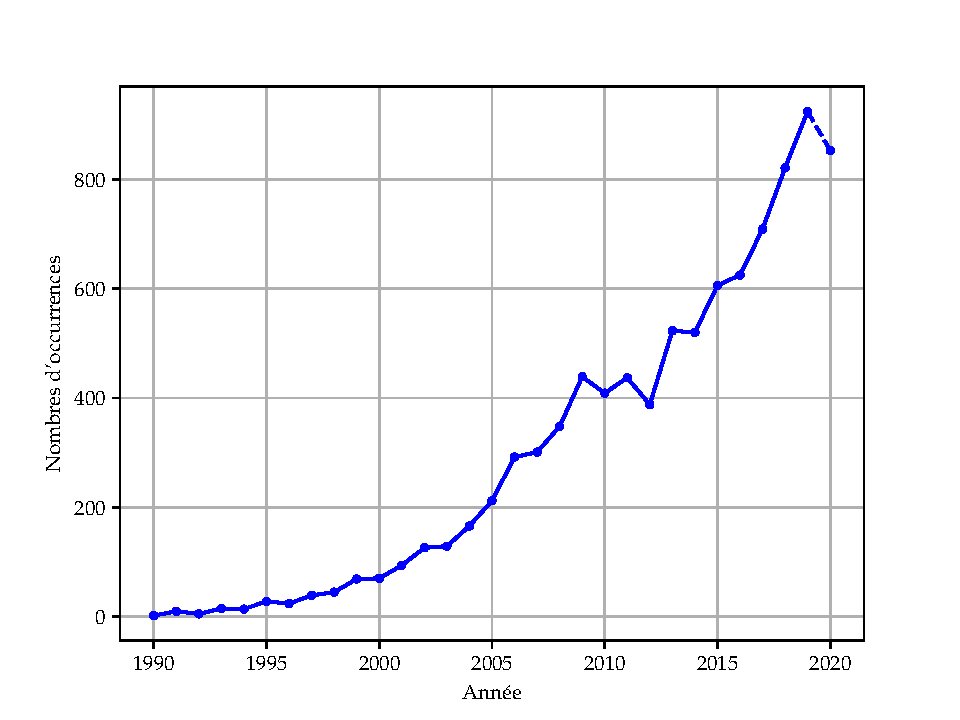
\includegraphics[width=\linewidth]{LBMocc} 
	\label{trend}
	\caption{Nombres de publications possèdent l'occurrence "Lattice Boltzmann Methods" répertoriées sur google scholar en fonction du temps.}
\end{figure}

%\begin{biography}{}{\author{Yohan Duarte} Biography text}
%\end{biography}

\end{document}
